\documentclass[fleqn,12pt,lineno,english]{wlpeerj}
\usepackage[T1]{fontenc}
%\usepackage[latin9]{inputenc}
%\usepackage{geometry}
\geometry{verbose,tmargin=1in,bmargin=1in,lmargin=1in,rmargin=1in}
%\usepackage{xcolor}
%\usepackage{verbatim}
\usepackage{float}
\usepackage{fancybox}
\usepackage{calc}
\usepackage{amssymb}
\usepackage{graphicx}
\usepackage{natbib}
\sloppy
\makeatletter

%\def\fps@figure{ht}

%%%%%%%%%%%%%%%%%%%%%%%%%%%%%% LyX specific LaTeX commands.
%% A simple dot to overcome graphicx limitations
\newcommand{\lyxdot}{.}
\newcommand{\otl}{OTLv4}
\newcommand{\otlprop}{OTLv4$^\prime$}
\newcommand{\supportedby}{\texttt{supported\_by}}
\newcommand{\partialpathof}{\texttt{partial\_path\_of}}
\newcommand{\terminal}{\texttt{terminal}}
\newcommand{\conflictswith}{\texttt{conflicts\_with}}
\newcommand{\resolves}{\texttt{resolves}}
\newcommand{\resolvedby}{\texttt{resolved\_by}}

\floatstyle{ruled}
\newfloat{algorithm}{tbp}{loa}
\providecommand{\algorithmname}{Algorithm}
\floatname{algorithm}{\protect\algorithmname}

%%%%%%%%%%%%%%%%%%%%%%%%%%%%%% User specified LaTeX commands.
\usepackage{algorithm,algpseudocode}
\usepackage{lmodern}
\usepackage{xcolor}
\usepackage{hyperref}
\hypersetup{
    colorlinks,
    linkcolor={red!50!black},
    citecolor={blue!50!black},
    urlcolor={blue!80!black}
}
\definecolor{mylime}{RGB}{128,255,128}

\@ifundefined{showcaptionsetup}{}{%
 \PassOptionsToPackage{caption=false}{subfig}}
\usepackage{subfig}
\makeatother

\usepackage{babel}
\global\long\def\taxonomy{\mbox{\ensuremath{\mathbb{T}}}}

\global\long\def\prunedTaxonomy{\taxonomy_{P}}

\global\long\def\phyloinputs{\mathcal{T}}

\global\long\def\expandedPhylo{\phyloinputs_{E}}

\global\long\def\summaryTree{\mathbb{S}}

\global\long\def\prunedSummary{\summaryTree_{P}}

\global\long\def\collections{\mathcal{C}}


\title{A supertree pipeline for summarizing phylogenetic and taxonomic information
for millions of species}

\author[1,2]{Benjamin D. Redelings}
\author[2,3,4]{Mark T. Holder}
\affil[1]{Department of Biology, Duke University, Durham NC, US}
\affil[2]{Department of Ecology and Evolutionary Biology, University of Kansas, Lawrence KS, US}
\affil[3]{Biodiversity Institute, University of Kansas, Lawrence KS, US}
\affil[4]{Heidelberg Institute for Theoretical Studies, Heidelberg, Germany}
\corrauthor[2,3,4]{Mark T. Holder}{mtholder@ku.edu}

% \keywords{Keyword1, Keyword2, Keyword3}

\begin{abstract}
We present a new supertree method that enables rapid estimation of a
summary tree on the scale of millions of leaves.  This supertree
method summarizes a collection of input phylogenies and an input taxonomy.
We introduce formal goals and criteria for such a supertree to satisfy
in order to transparently and justifiably represent the input
trees. In addition to producing a supertree, our method computes
annotations that describe which grouping in the input trees support
and conflict with each group in the supertree. 

\medskip

We compare our supertree construction method to a previously published
supertree construction method by assessing their performance on input
trees used to construct the Open Tree of Life version 4, and find that
our method increases the number of displayed input splits from 35,518
to 39,639 and decreases the number of conflicting input splits from
2,760 to 1,357.  The new supertree method also improves on the previous
supertree construction method in that it produces no unsupported
branches and avoids unnecessary polytomies. 

\medskip

This pipeline is currently used by the Open Tree of Life project to
produce all of the versions of project's ``synthetic tree'' starting
at version 5.This software pipeline is called
\emph{``propinquity.''}. It relies heavily on \emph{``otcetera''} - a
set of C++ tools to perform most of the steps of the pipeline. All of
the components are free software and are available on GitHub.
\end{abstract}

\begin{document}

\flushbottom
\maketitle
\thispagestyle{empty}

\section{Background}

The Open Tree of Life project seeks to build a platform for summarizing
what is known about phylogenetic relationships across all of Life
\citep{HinchliffEtAl2015}. One primary goal of the project is to
build a summary tree from a comprehensive taxonomic tree and a set
of published trees. The summary tree is intended to transparently
and justifiably represent phylogenetic information from these inputs.
The taxonomic tree is derived from the Open Tree Taxonomy (OTT hereafter,
publication in preparation). The phylogenetic inputs are published
trees that have been curated to align the tips to OTT and to identify
the correct rooting (see \citealt{McTavishEtAt2015} for further details
of the curation tools). Unlike OTT, these phylogenetic trees do not
include all leaf taxa. The inputs (taxonomy and phylogenetic trees)
and the output summary supertree are all rooted. Here we describe
the software pipeline (\emph{propinquity}) that summarizes and integrates
these smaller source trees and the taxonomy tree into a single supertree
and the noteworthy tools for manipulating and solving supertrees in
the \emph{otcetera} package.

\subsection{Goals}

Translating the goals of the Open Tree of Life's summary tree into
an explicit set of criteria is not trivial. The summary supertree
should represent the phylogenetic information from source trees in
a transparent and justifiable fashion. We would like to allow users
to correct errors in the supertree by improving the input information
rather than requiring modification to the supertree algorithm. The
pipeline was designed to create a tree which:
\begin{enumerate}
\item displays no unsupported groups,
\item defers to groupings from higher ranked trees in the case of conflict, 
\item contains no unnecessary polytomies, and
\item displays as many groupings from input trees as possible.
\end{enumerate}
These goals are described more fully below. In order to accomplish
transparency and justification, our pipeline also produces annotations
files with information about conflict and support. 

\subsubsection{Goal 1: Each grouping is supported by at least one input}

We require that each edge in the supertree be supported by at least
one input tree edge. In addition to aiding interpretability, this
requirement keeps the supertree from arbitrarily representing information
that comes from none of the input trees. Of course, in a supertree
analysis, the full tree will imply some relationships for subsets
of the taxa that are not found in any input tree. So, the meaning
of ``supported by'' needs some clarification. 

\paragraph*{Notation, terminology, and the definition of ``supported by''}

Let $\summaryTree$ denote a supertree, and $T_{i}$ denote the $i$th
input tree. The set of taxa that are mapped to the tips of the tree
$T_{i}$ is $\mathcal{L}(i)$. $\summaryTree(i)$ denotes the summary
tree induced by tip nodes that are mapped to taxa in $\mathcal{L}(i)$
and the most recent common ancestor of those leaves, and any other
node that is an ancestor of some but not all of these leaves. We say
that edge $j$ of the supertree is compatible with an input tree,
$T_{i}$ if edge $j$ either is not included in the induced tree $\summaryTree(i)$
or none of the edges in $T_{i}$ are in conflict with edge $j$ in
the induced tree. 

We can consider whether or not a node in an input tree is displayed
by $\summaryTree$. For any such node $j$ there is a set of taxa
that are mapped to the tips that descend from the node. This set of
taxa is the ``cluster'' of taxa corresponding to node $j$; it can
be denoted $\mathcal{L}(i,j)$. It will also be referred to as the
``include set'' of the node. The ``exclude set'' of $j$ in $T_{i}$
is the set of taxa in $\mathcal{L}(i)$ but not in $\mathcal{L}(i,j)$.
If the cluster of taxa for any supertree node in $\summaryTree(i)$
is identical to $\mathcal{L}(i,j)$, then we say that $\summaryTree$
displays node $j$ of $T_{i}$. We say that the summary tree \emph{displays}
edge $j$ if the summary tree displays the child node of edge $j$.
Operationally, we can find the most recent common ancestor (MRCA)
node of $\mathcal{L}(i,j)$ in $\summaryTree$; the summary tree displays
$j$ if and only if that MRCA node is not an ancestor of any member
of the exclude set of $j$. We say that node $k$ of the summary tree
is \emph{supported by} node $j$ in $T_{i}$ if the summary tree displays
node $j$, but if we contracted edge that separates $k$ from its parent then the modified summary
tree would no longer display node $j$. 

Note that stating that a node in the summary tree is supported by
an input does not imply that every descendant of that node must be
present in the input nor that every taxon that is not a descendant
must be excluded in order to display the node. Consider the problem
shown in figure \ref{fig:toyambig}; panels (\ref{fig:toyambig}a)
and (\ref{fig:toyambig}b) show two input trees. Because taxa A and
E do not occur together in either input, there is some uncertainty
about where to place them. By our terminology, either output shown
in (\ref{fig:toyambig}c) or (\ref{fig:toyambig}d) would be characterized
as a tree that displays all of the input groupings and which has no
unsupported groups. Clearly these criteria are insufficient to specify
a unique solution, and users of the output tree need to be aware that
it may be possible for some taxa to ``float'' to multiple positions.
In figure \ref{fig:toyambig}, taxon E floats to different positions
in (\ref{fig:toyambig}c) and (\ref{fig:toyambig}d), whereas taxon
A does not. 

\begin{figure}
\subfloat[Input tree 1]{\includegraphics[width=0.45\textwidth]{Figures__toy_ambig__abcd}

}\hfill{}\subfloat[Input tree 2]{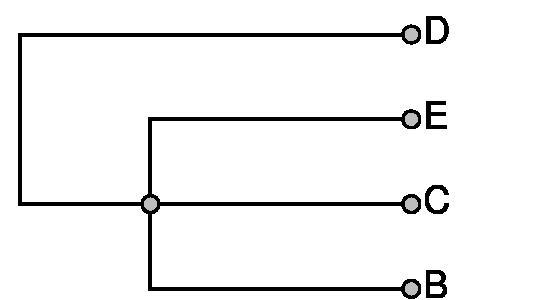
\includegraphics[width=0.45\textwidth]{Figures__toy_ambig__bcde}

}

\subfloat[Summary tree]{\includegraphics[width=0.45\textwidth]{Figures__toy_ambig__soln1}

}\hfill{}\subfloat[Summary tree]{\includegraphics[width=0.45\textwidth]{Figures__toy_ambig__soln2}

}

\caption{An example demonstrating that our definition of ``supported by''
does not imply entire composition of a grouping. (a) and (b) show
2 input trees and (c) and (d) depict trees that each display each
of the groupings in the input trees and which have no unsupported
nodes. The BUILD algorithm (section \ref{fig:subproblem-solutions.})
would choose tree (d) that floats taxon E closer to the root.}

\label{fig:toyambig}
\end{figure}

One of our aims in supertree construction is to minimize the amount
of information in the supertree that does not come from input trees.
We permit information that comes from combinations of input trees,
but not any single input tree. However, we seek to exclude information
that comes from none of the input trees. This motivates the criterion
of not having any unsupported edges, since these edges could be removed
without decreasing the support from any input tree.

\subsubsection{Goal 2: Tree ranking}

An appealing goal for the summarization would be to find the supertree
that displays the largest number of input tree edges. As discussed
in \citet[pages 92 and 131;][]{HusonRS2010} the maximum compatibility
problem is known to be $NP$-hard via a reduction to Max-Clique \citep{Karp1972}.
In addition to being computationally daunting, this formulation of
the supertree problem does not provide biologists who use the summarization
tool with an obvious avenue for fixing perceived problems with the
summary tree. For example, a grouping that a biologist expected may
not be present in the supertree, but it may not conflict with any
of the input groupings which are displayed. This can happen because
displaying both node $a$ from $T_{1}$ and node $b$ from tree $T_{2}$
in a summary tree may only be possible by displaying a grouping that
is present in no input tree. All other factors being equal, if this
implied grouping conflicts with input node $c$ in tree $T_{3}$,
then $c$ will not be displayed in the summary tree, but a biologist
will not necessarily know how to fix this problem. One solution is
to use a ranking of groupings. If an expert were quite confident in
the $c$ grouping, then she could assign that input node a high ranking.
A supertree that used ranks could then recover this grouping even
if its inclusion did not increase the total number of input nodes
that are displayed by the summary tree. Figure (\ref{fig:pairwisecompat})
shows an example of 3 input trees for which there is no pairwise incompatibility,
but no solution displays all of the input groups. Alternative rankings
of inputs can result in one of three summary trees shown in panels
(d-f). 

\begin{figure}
\subfloat[Input tree 1]{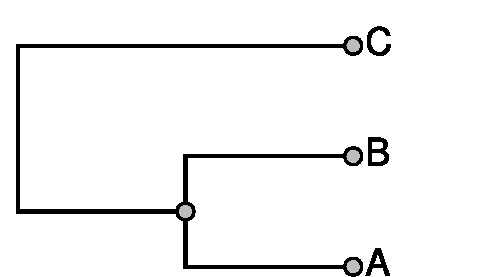
\includegraphics[scale=0.57]{Figures__toy_pairwise_compat__abc}

}\hfill{}\subfloat[Input tree 2]{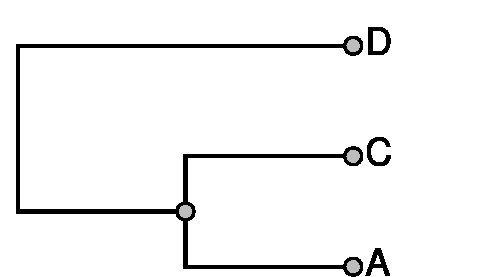
\includegraphics[scale=0.57]{Figures__toy_pairwise_compat__acd}

}\hfill{}\subfloat[Input tree 3]{\includegraphics[scale=0.57]{Figures__toy_pairwise_compat__bcd}

}

\subfloat[Summary tree]{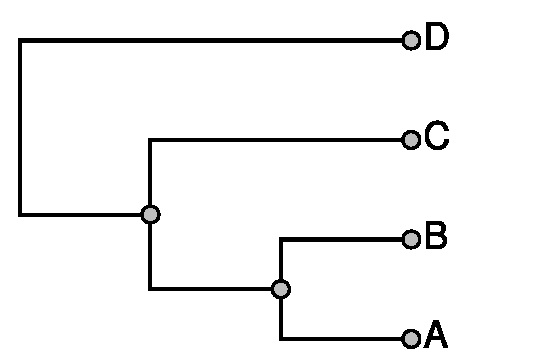
\includegraphics[scale=0.57]{Figures__toy_pairwise_compat__s12}

}\hfill{}\subfloat[Summary tree]{\includegraphics[scale=0.57]{Figures__toy_pairwise_compat__s13}

}\hfill{}\subfloat[Summary tree]{\includegraphics[scale=0.57]{Figures__toy_pairwise_compat__s23}

}

\caption{An example of 3 input trees shown in (a), (b), and (c) which do not
conflict in a pairwise manner, but cannot be jointly displayed in
one tree. The 3 solution trees are shown in panels (d-f). Panel (d)
for ranking the tree in (c) lowest. Panel (e) shows the solution if
the tree in (b) has the lowest rank. Panel (f) shows the solution
if the tree in (a) is ranked lowest. Each of the solutions displays
2 of the 3 input groupings. }

\label{fig:pairwisecompat}
\end{figure}

Any approach to supertree construction must deal with the need to
adjudicate between conflicting input trees. We choose to deal with
conflict by ranking the input trees, and preferring to include edges
from higher-ranked trees. The merits of using tree ranking are questionable
because the system does not mediate conflicts based on the relative
amount of evidence for each alternative. However, it is a reasonable
starting point. It has the benefits of making it easy to see why some
groups are included or not (transparency), and it allows simpler and
cleaner algorithms.

Note that if some edge $c$ conflicts with a higher-ranked edge $b$,
then $c$ may still be included in the supertree. This can occur when
the higher ranked edge $b$ conflicts with a yet-higher ranked edge
$a$, and thus $b$ is not included. In that case, it will be possible
for $c$ to be represented in the summary tree. Thus, the fact that
the summary tree displays an input edge does not imply that none of
the higher ranked input trees conflict with that edge. 

In order to produce a comprehensive supertree, we also require a rooted
taxonomy tree in addition to the ranked list of rooted input trees.
Unlike other input trees, the taxonomy tree is required to contain
all taxa, and thus has the maximal leaf set. We make the taxonomy
tree the lowest ranked tree. In our current formulation, the taxonomy
tree is also unique in that the taxonomy is the only source of taxonomic
names. Each node in the taxonomy tree corresponds to a named group.
Taxonomic groups may have the same name, but each node in the taxonomy
tree is identified by a unique number (its OTT ID). Taxonomic groups
are identified in the summary supertree by finding a branch (or ``node'')
that has exactly the same include|exclude relationship. The taxonomy
supertree can meaningfully possess degree-two nodes. Although these
nodes can be removed without affecting the relationships of the leaves,
they do represent nested taxonomic groups that contain exactly one
subgroup. The taxonomy is also used to determine which tips are terminal
taxa.

\subsubsection{Goal 3: Contain no unnecessary polytomies}

The supertree should be as resolved as possible - in other words,
it should have no unnecessary polytomies. Thus, for each input edge
that is \emph{not} included, we can point to a reason for non-inclusion
by showing that the input edge conflicts with some edge of the summary
tree. Note, that the requirement to not display unsupported groups
leads to some ``necessary'' polytomies. For example any resolution
of the polytomy shown in figure (\ref{fig:pairwisecompat}e) would
continue to display the same two input groups. However, the additional
grouping would be unsupported, because the unresolved tree already
displays both input groups. Thus, the 
unresolved tree would be preferred by our criterion.
However, collapsing either internal edge of the tree shown in figure
(\ref{fig:pairwisecompat}d) would result in a tree which displays
only one input grouping. This tree would contain an unnecessary polytomy,
because the polytomy would permit refinement to the depicted tree
which displays more input groupings.

\subsubsection{Goal 4: Display as many input nodes as feasible}

We also seek to construct a supertree that represents as many input
tree nodes as possible. Since non-included input tree nodes must conflict
with the supertree (or they would have been added), this criterion
is the same as minimizing the number of input nodes that conflict
with the supertree.

\subsubsection{Summary of goals}

These optimality criteria help to define what it means for the supertree
to represent the input trees, as well as justifying and explaining
why various features of the supertree exist. The pipeline described
below produces a supertree that satisfies the first three optimality
criteria and is a greedy approximation of a solution to the fourth
goal. It is not guaranteed to display as many input nodes as possible.
Even if the summary tree does accomplish goal 4, it is not necessarily
a \emph{unique} optimum. The pipeline takes a greedy approach to producing
a summary tree by attempting to add groupings from the trees in order
of the trees ranking. This can be viewed as a greedy solution to the
problem of finding the tree with the maximum sum of displayed groups'
weighted scores criterion (MSDGWS, described in the appendix A) where the
weights from the trees are so extreme that displaying one group from
a highly ranked tree is preferred to displaying all of the groupings
from lower ranked trees.

\section{Description of the supertree method}

\subsection{Preprocessing steps}

Propinquity was designed to function as a part of the Open Tree of
Life software architecture, so the first few steps of the pipeline
involve transforming artifacts from that project into a set of rooted
trees and a phylogenetic taxonomy. The phylesystem API \citep{McTavishEtAt2015}
of Open Tree allows users to curate published estimates of trees and
create ranked collections of these trees. Early steps in the propinquity
pipeline manipulate the phylogenetic input trees to improve their
usability and reliability. The first steps of the pipeline (see Figure
\ref{fig:pipeline}) collect a list of trees to include (in the \texttt{phylo\_input}
subdirectory) and store copies of these files (in the \texttt{phylo\_snapshot}
subdirectory) to make it easier to replicate the operation (because
the collection of trees and the tree files change due to curation).
\begin{figure}
\begin{centering}
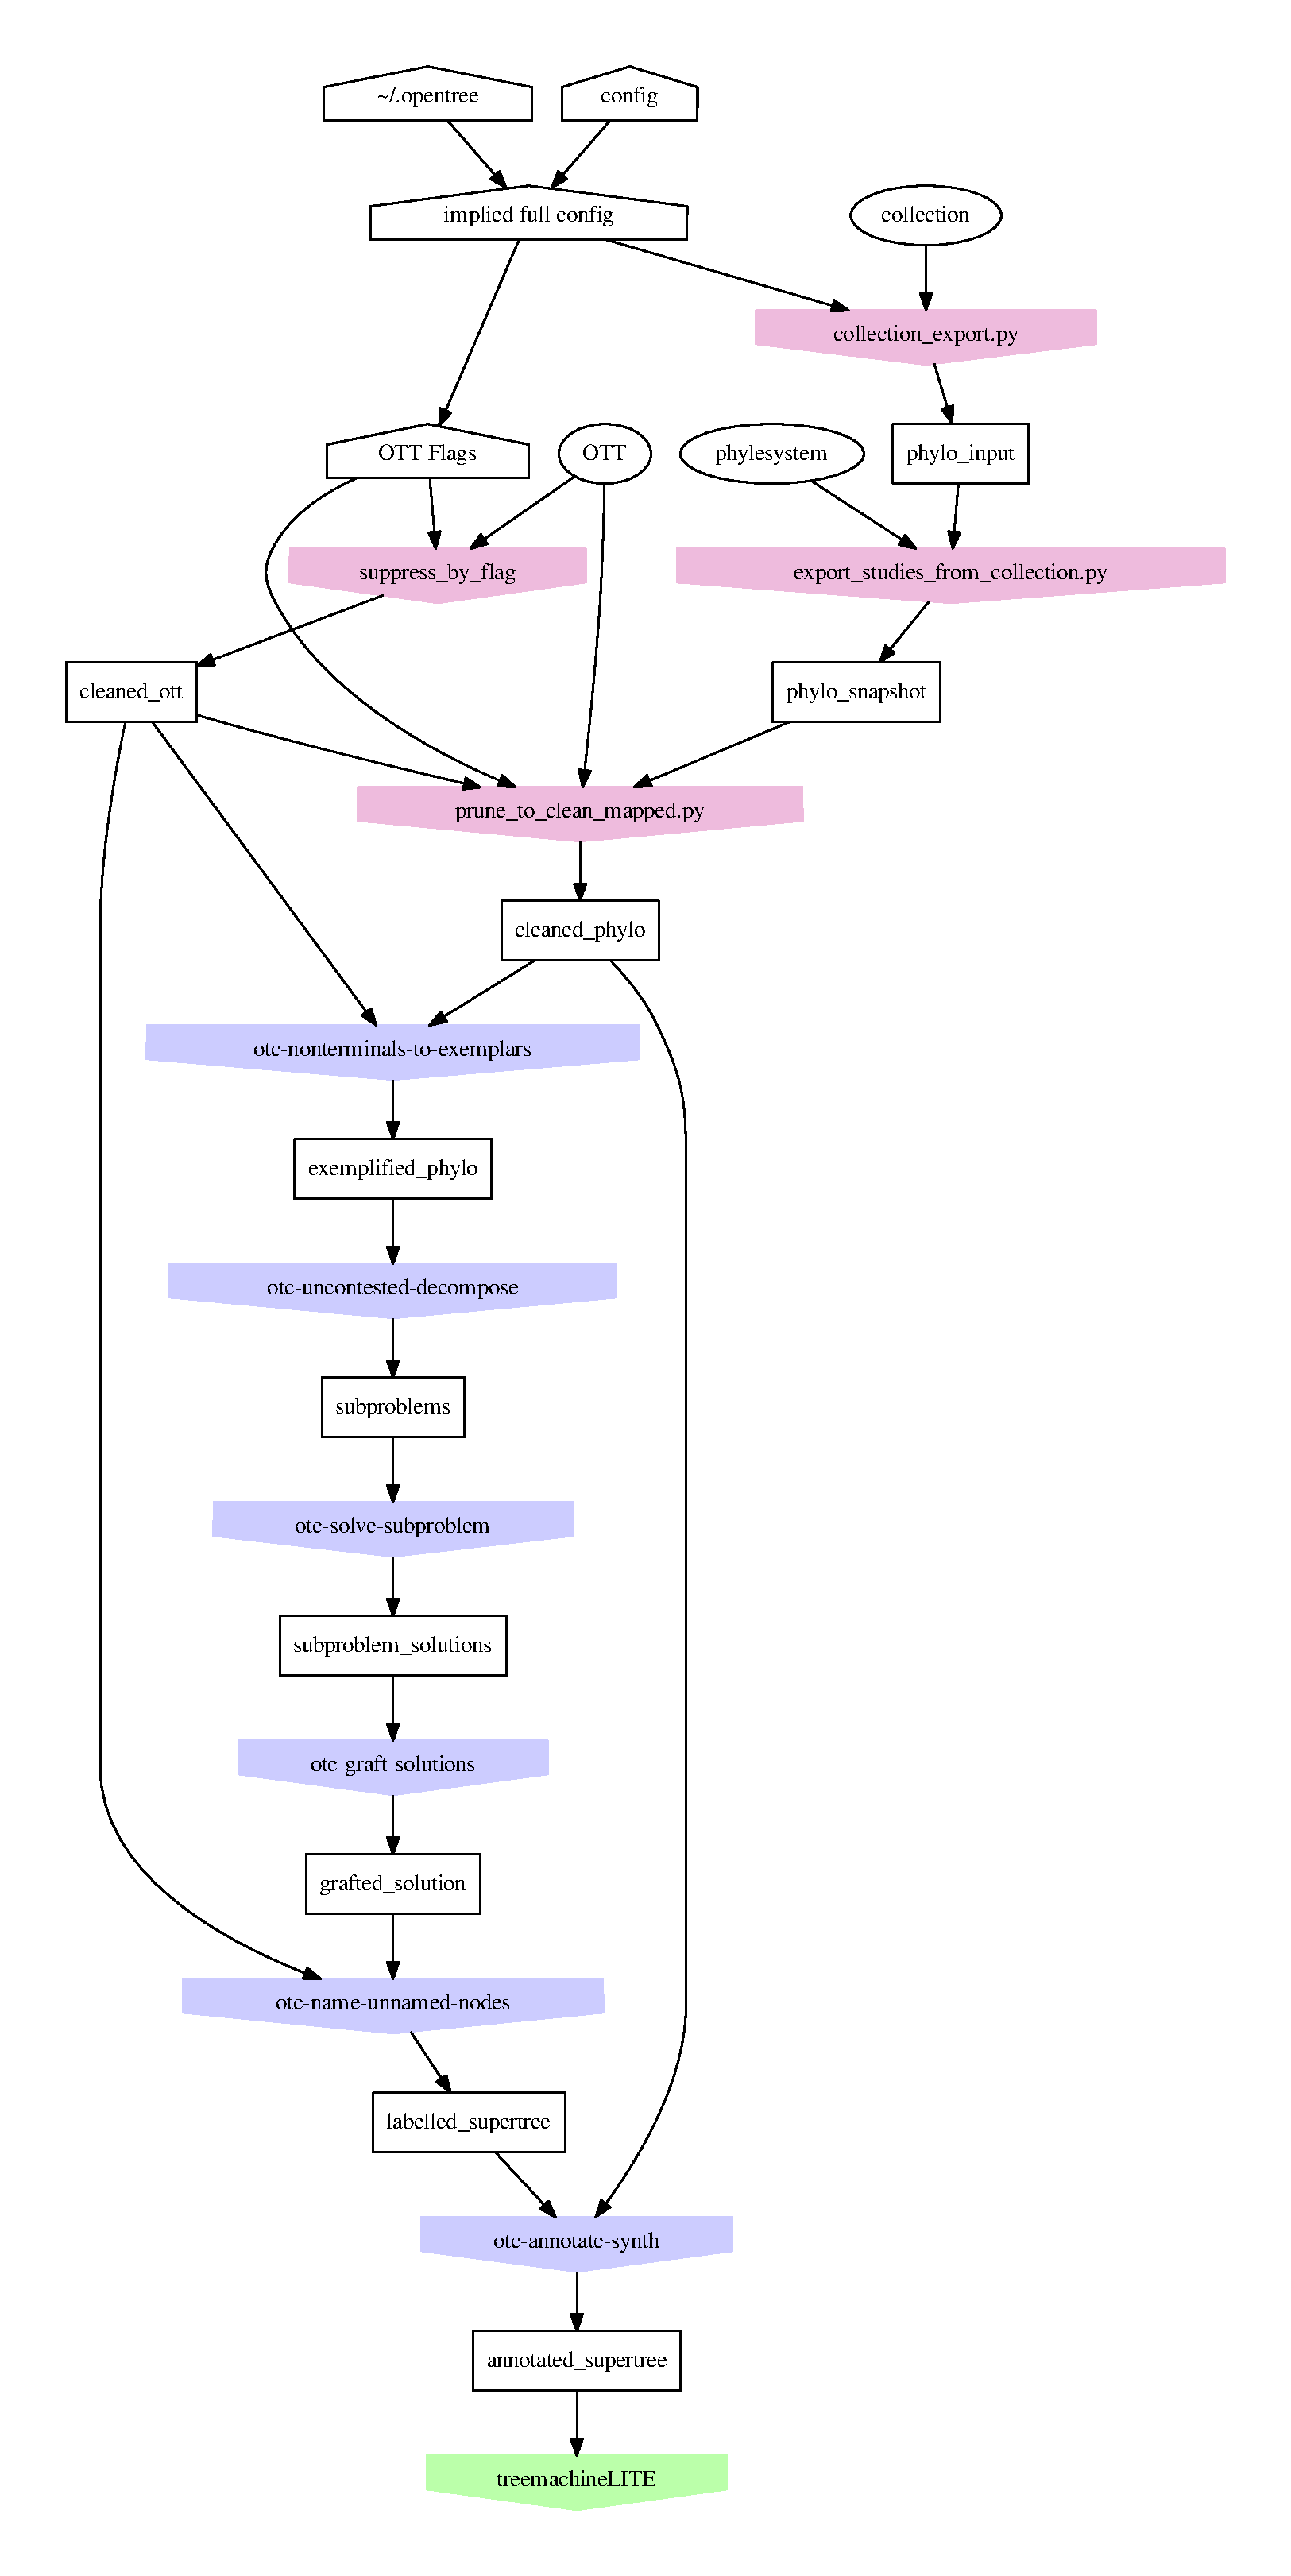
\includegraphics[height=0.75\paperheight]{pipeline-tools.pdf}
\par\end{centering}
\caption{Organization of the \emph{propinquity} pipeline. Each colored pentagon
labels a program (blue for otcetera-based tools and red for python
scripts in the propinquity or peyotl repository) that performs the
important operations in each step; the number before the tool name
refers to the section in this paper that describes the operation.
The output of each step corresponds to a subdirectory of the propinquity
system which will hold the output artifacts for the step. Ovals are
resources that are required (OTT and Open Tree's phylesystem repository).
White pentagons are user-controlled inputs.}
\label{fig:pipeline}
\end{figure}


\subsubsection{Pruning questionable taxa from the taxonomy}

OTT is a hierarchy of taxonomic names that implies a phylogenetic
taxonomy. An OTT ID has a position in the hierarchy, a taxonomic name,
and set of references to the same name in different taxonomies. In
addition, the ID may also be associated with a set of flags that can
indicate that the taxon may be questionable. These flags can either
encode information taken from an input taxonomy (for example, taxa
the NCBI refers to as ``unplaced'' are assigned an ``unplaced''
flag) or can arise because of some form of conflict during taxonomy
construction (for example, if two taxonomies disagree on the name
for a taxon, then the taxon can be merged and the name will be retained
without any descendants; this name will have an OTT ID, but will be
flagged as ``barren''). Propinquity prunes the OTT down to a more
reliable taxonomy by pruning off parts of the tree that are flagged
with suspicious flags. The set of flags that lead to a subtree of
the taxonomy being pruned is under the control of the user (the set
of flags used by the Open Tree of Life project can be found in the
\texttt{config.opentree.synth} file in the propinquity repository).
For the purpose of the rest of the pipeline, an OTT ID that has been
pruned from the taxonomy will be treated in the same way as invalid
OTT ID. The output of this step is stored in propinquity's \texttt{cleaned\_ott}
subdirectory; this operation only needs to be performed when the OTT
or the pruning flags change.

\subsubsection{Pruning problematically mapped tips from input phylogenetic trees}

Frequently, phylogenetic estimates are rooted using the outgroup criterion,
which is an assumption about the monophyly of the ingroup taxa. Because
the rooting of the branches in the outgroup portion of the tree is
often uncertain, data curators can identify the ingroup node of the
tree; propinquity uses this annotation to prune off the outgroup taxa.

Frequently, not all tips in a phylogenetic input will have been mapped
to a taxon in the current version OTT. Unmapped leaves are pruned
from each phylogenetic input. In some cases, the OTT has changed and
a taxon has been unambiguously mapped to another taxon. This can occur
when multiple species in one version of the taxonomy are ``lumped''
into a single taxon in a subsequent version. OTT maintains a set of
``forwarding'' statements about IDs that have been removed but can
be mapped to an existing taxon; propinquity uses these statements
to update the OTU mapping of input trees.

Finally some leaves are mapped to taxa that occur more than once in
the tree, or taxa that have ancestors represented as tips of the tree.
In these cases, leaves are pruned to assure that tips are mapped to
unique taxa that are not nested. In the case of nested taxa, the tip
mapped to the higher level taxon is pruned, and one of the lower level
tips is retained. In the case of duplicate occurrences of an OTT taxon,
propinquity checks to see if a data curator has selected one of the
taxa to be the exemplar for the taxon. If this selection has not been
made, then the node with the lexicographically lowest ID is chosen
to exemplify the taxon. This choice is arbitrary, but repeatable.
The pruned phylogenetic inputs are stored in a \texttt{cleaned\_phylo}
subdirectory of propinquity.

\subsubsection{Exemplifying tips mapped to higher taxa}

Many input trees have tips that are not terminal taxa, but higher-order
taxonomic groups. It is not clear how to interpret a tip in a phylogenetic
estimate that is labeled with the name of a higher taxon. Several
scenarios can lead to these cases: the data for the tip could have
been created by merging a chimeric set of character scores from constituent
taxa; the species sampled may not have been identified to the lowest
taxonomic rank; or the researcher may simply have used a higher taxonomic
name because he/she assumed that the taxon is monophyletic and the
higher level name would be more recognizable. Rather than allowing
the ambiguity about interpretation of the higher-taxon mapped tips
to propagate throughout the entire pipeline, we transform the input
trees by replacing higher taxa at tips with a set of terminal-taxon
exemplars for each taxon. One approach would be to simply determine
all descendant terminal taxa and attach them as children of the problematic
tip. However, this would create a clade rather than a tip; subsequent
steps in the supertree would interpret the clade as a claim of monophyly
for the taxon. The input tree may not have tested monophyly of the
clade, so this interpretation is unwarranted. We avoid it by attaching
exemplar taxa as child nodes of the higher taxonomic tip but then
collapsing the edge between the former tip node and
its parent. Thus, if $A$ is a non-terminal taxon containing terminal
descendants $a_{1}$ and $a_{2}$ and $B$ is a non-terminal taxon
containing terminal descendants $b_{1}$ and $b_{2}$ we would replace
the subtree $((A,B),c)$ with $((a_{1},a_{2},b_{1},b_{2}),c)$ instead
of the subtree $(((a_{1},a_{2})A,(b_{1},b_{2})B),c)$.

If a taxon is only present in the taxonomy (not in any of the input
trees), then it can be pruned from the taxonomy for the construction
of the supertree and then grafted back on to the summary tree later.
Performing this pruning reduces the size of the supertree problem,
reducing the running time of the pipeline. Similarly, when we expand
a higher taxon in the exemplification step, we can omit members of
the taxon if they do not occur in any of the phylogenetic inputs.
If there are no members of the higher taxon sampled in any other input
tree, then we arbitrarily choose one terminal taxon to represent the
higher taxon. During the exemplification step, a tool from otcetera
(\texttt{otc-nonterminals-to-exemplars}) reads the taxonomy and all
of the ``cleaned'' phylogenetic estimates from the previous step.
Reading all of the inputs is necessary to assure that each higher
taxon is replaced with the same set of exemplars regardless of which
tree the higher taxon occurs in, and that the exemplars for a higher
taxon is the union on the set of descendant terminal taxa that have
been sampled in a phylogenetic input. Figure \ref{fig:exemplify-example}
shows an example of how the trees in figure \ref{fig:cleaned-phylo-example}
would be exemplified.

We prune the taxonomy by removing tips that are not present in any
input tree to produce the pruned taxonomy $\mathbb{T}_{p}$. The tips
pruned in this step will be grafted back onto the skeleton of the
summary tree in a subsequent step. A terminal taxon that is represented
only in the taxonomy can be pruned and then regrafted onto the solution
without affecting which nodes are displayed by the final summary tree.
Thus, this procedure does not impede our ability to find a good summary
tree. Removing these tips produces a smaller input to the rest of
the pipeline, which reduces running times. After producing the set
of ``exemplified'' phylogenetic inputs, this tool exports a pruned
down version of the taxonomy that only contains tips that are present
in at least one phylogenetic input.

\begin{figure}
\subfloat[Tree 1]{\includegraphics[scale=0.4]{Figures__cleaned_phylo__ex_2@tree1\lyxdot tre}

}\hfill{}\subfloat[Tree 2]{\includegraphics[scale=0.4]{Figures__cleaned_phylo__ex_2@tree2\lyxdot tre}

}\hfill{}\subfloat[Taxonomy Tree]{\includegraphics[scale=0.4]{Figures__cleaned_ott__cleaned_ott\lyxdot tre}

}

\caption{Input trees and taxonomy tree}
\label{fig:cleaned-phylo-example}
\end{figure}
 
\begin{figure}
\subfloat[Tree 1]{\includegraphics[scale=0.4]{Figures__exemplified_phylo__ex_2@tree1\lyxdot tre}

}\hfill{}\subfloat[Tree 2]{\includegraphics[scale=0.4]{Figures__exemplified_phylo__ex_2@tree2\lyxdot tre}

}\hfill{}\subfloat[Pruned taxonomy tree $\protect\prunedTaxonomy$]{\includegraphics[scale=0.4]{Figures__exemplified_phylo_taxonomy_uncontested\lyxdot tre}

}

\caption{Exemplified input trees and taxonomy tree from figure \ref{fig:cleaned-phylo-example}.
E in tree1 is exemplified by E1. Pruned taxa are E2, F2, and D. The
taxa E and F are retained as monotypic taxa in the pruned taxonomy
$\protect\prunedTaxonomy$, but are not shown in panel c. The red
edge in the pruned taxonomy tree is an uncontested higher taxon in
the exemplified taxonomy (as explained in section \ref{subsec:Subproblem-decomposition})}
\label{fig:exemplify-example}
\end{figure}


\subsection{Summary tree construction}

After the preprocessing steps, the inputs have been converted to a
set of rooted phylogenetic estimates in which each leaf is mapped
to a terminal taxon in the exemplified taxonomic tree. The goal of
the remainder of the pipeline is to construct a tree that maximizes
the sum of displayed groups' weighted scores (MSDGWS) criterion. This is accomplished
in four steps: (1) dividing the full problem into subproblems based
on uncontested taxa, (2) constructing a summary solution for each
subproblem by greedily creating a maximally-sized list of groupings
that can all be displayed simultaneously; (3) grafting the subproblem
solutions into a single supertree; and (4) grafting (or ``unpruning'')
the taxonomy-only taxa onto the solution to produce a complete summary
tree.

\subsubsection{Subproblem decomposition\label{subsec:Subproblem-decomposition}}

For the sake of efficiency, propinquity uses a divide-and-conquer
approach to construct the supertree. Subproblems are identified by
searching through the taxonomy tree to find any taxa that are not contested
by any single input tree. Here we say that input tree $T_{i}$ contests
taxon $x$ in the pruned taxonomy, if $x$ is not monophyletic in
any resolution of tree $T_{i}$. Thus, polytomies in an input tree
are treated as soft polytomies, and a taxon is not contested merely
because it is not displayed by an input tree. 

This operation is performed by the \texttt{otc-uncontested-decompose}
tool in otcetera; see appendix \ref{sec:Decompose-algorithm} for
a description of the algorithm. The output is a series of subproblems,
each of which corresponds to a slice of the taxonomy and corresponding
slices through each relevant input tree. Each uncontested non-terminal
and non-root taxon will show up in two subproblems: it will be the
root of its own subproblem and it will be tip in the subproblem that
covers the next slice deeper in the tree. The red edge in figure \ref{fig:exemplify-example}c
highlights the taxa that are not contested by the input shown in \ref{fig:exemplify-example};
figure \ref{fig:subproblems-example} shows the subproblems that would
be emitted as a result of this set of inputs. The supertree operation
of \citet{HinchliffEtAl2015} also used this otcetera-based decomposition
step.

Note that decomposition into uncontested groups does not necessarily
allow us to find the tree that maximizes the MSDGWS score. For example,
see figure \ref{fig:decompose-worsens}; that example is a variant
of the situation shown in figure \ref{fig:pairwisecompat}. In this
case the groupings from each of the phylogenetic estimates, shown
in panels \ref{fig:decompose-worsens}a and \ref{fig:decompose-worsens}b,
could be displayed. That solution is shown in panel \ref{fig:decompose-worsens}d,
it displays two of the three input splits, but is optimal because
no solution displays all three input groupings and the depicted solution
displays the two highest ranked groupings. However, neither of the
trees shown in panels \ref{fig:decompose-worsens}a or \ref{fig:decompose-worsens}b
contest the taxon $B$ shown in the taxonomy panel \ref{fig:decompose-worsens}c.
Thus, when using our decomposition, the branches leading to taxa $B1$
and $B2$ in the input phylogenetic trees would be sliced during the
decomposition, and relabeled to refer to taxon $B$. This taxonomically-informed
interpretation of the inputs views the two phylogenetic inputs as
in conflict; so the solution returned by propinquity would defer to
the higher ranked tree. The tree shown in panel \ref{fig:decompose-worsens}e
would be returned. This example arises from the fact that the trees
in \ref{fig:decompose-worsens}a and \ref{fig:decompose-worsens}b
jointly contest taxon $B$, but neither contests taxon $B$ when the
trees are considered in isolation.

Despite the fact that the use of \texttt{otc-uncontested-decompose}
can worsen the final score of the summary tree, we use this approach
in propinquity because it makes the construction of the tree faster
and it is easy for users to correct issues caused by incorrect taxa
being constrained to be monophyletic. By adding a tree (even a low-ranked
tree) that contests a taxon to the corpus of input trees , then the
next synthetic tree will no longer consider the taxon to be uncontested.
Thus the procedure encourages curation of more phylogenetic inputs
as a means of improving the summary tree. 

\begin{figure}
  \subfloat[Subproblem \emph{ABCD}]{\includegraphics[width=0.3\textwidth]{Figures__subproblems__14__1\lyxdot tre}%
    \hfill{}\includegraphics[width=0.3\textwidth]{Figures__subproblems__14__2\lyxdot tre}%
    \hfill{}\includegraphics[width=0.3\textwidth]{Figures__subproblems__14__3\lyxdot tre}

}

  \subfloat[Subproblem \emph{root}]{\includegraphics[width=0.3\textwidth]{Figures__subproblems__17__1\lyxdot tre}%
    \hfill{}\includegraphics[width=0.3\textwidth]{Figures__subproblems__17__2\lyxdot tre}%
    \hfill{}\includegraphics[width=0.3\textwidth]{Figures__subproblems__17__3\lyxdot tre}

}

\caption{Subproblems generated from the exemplified trees shown in figure \ref{fig:exemplify-example}.
A trivial statemen from the first tree that a taxon labelled $ABCD$
is sister to $E$ has been omitted, because trees with only 2 leaves
do not contain phylogenetic information.}
\label{fig:subproblems-example}
\end{figure}
\begin{figure}
\subfloat[]{\includegraphics[scale=0.57]{Figures__uncontested_worsens_score__ab1c}

}\hfill{}\subfloat[]{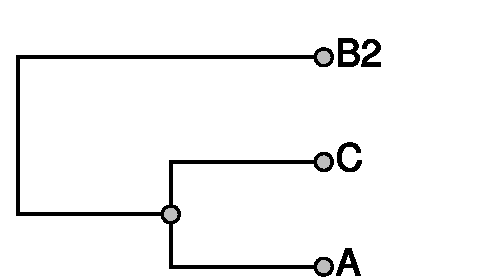
\includegraphics[scale=0.57]{Figures__uncontested_worsens_score__acb2}

}\hfill{}\subfloat[]{\includegraphics[scale=0.57]{Figures__uncontested_worsens_score__tax}

}

\hfill{}\subfloat[]{\includegraphics[scale=0.57]{Figures__uncontested_worsens_score__opt}

}\hfill{}\subfloat[]{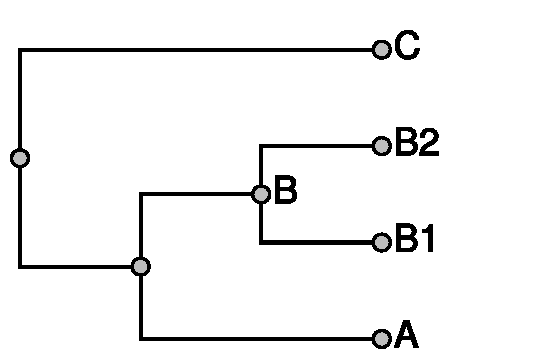
\includegraphics[scale=0.57]{Figures__uncontested_worsens_score__returned}

}\hfill{}

\caption{An example with three input trees: the highest ranked phylogenetic
input panel (a), the second ranked phylogenetic input (b), and the
taxonomy in panel (c). The summary tree in panel (d) has the highest
possible score, but the summary shown in panel (e) would be returned
from the pipeline that uses uncontested taxon decomposition.}
\label{fig:decompose-worsens}
\end{figure}


\subsubsection{Subproblem solution\label{subsec:Subproblem-solution}}

When solving sub-problems, we sequentially incorporate splits from
trees in order of ranking, retaining splits that are compatible with
the current set of splits (Alg \ref{alg:ConsistentSplitsFromRankedList}).
The order of splits from the same tree is not specified by this approach,
and we incorporate splits using one of the possible post-order traversals
of the tree. We make use of the BUILD algorithm \citep{AhoSSU1981}
to assess compatibility. This strategy avoids unnecessary polytomies,
since splits of later input trees are only rejected from the summary
supertree if they conflict with higher-priority splits. Finally, we
use the BUILD algorithm to construct a supertree displaying all of
the splits in the set of compatible splits. Using the BUILD algorithm
to construct the subproblem summary tree satisfies criterion 3, because
trees from the BUILD algorithm do not contain unsupported branches.
\begin{algorithm}
\begin{algorithmic}
\Require An ordered list of $M$ splits, $\mathcal{R} = [R_1, R_2, R_3, \ldots, R3, \ldots, R_M]$
\State $\mathcal{C} = [R_1]$
\For{each split $i$ in $[2, 3 \ldots M]$}
   \State $\mathcal{T} \leftarrow \mathcal{C} + R_i$ \Comment{where `+' means concatenating 2 lists}
   \If{\textsc{BUILD}$(\mathcal{T})$ does not return null}
      \State $\mathcal{C} \leftarrow \mathcal{T}$
   \EndIf
\EndFor{}
\State\Return $\mathcal{C}$
\end{algorithmic}

\caption{\label{alg:ConsistentSplitsFromRankedList}ConsistentSplitsFromRankedList}
\end{algorithm}

The BUILD algorithm as originally stated by \citet{AhoSSU1981} applies
to a collection of rooted triplets. Instead of decomposing each input
split into a collection of rooted triplets, we instead modify the
BUILD algorithm to apply directly to larger rooted splits. The modified
BUILD algorithm constructs a tree compatible with a collection of
rooted splits, and returns failure if such a tree does not exist.
This modified algorithm recovers the original BUILD algorithm if only
rooted triplets are supplied as input. When larger splits are supplied
as input, the results are the same as if each was was decomposed into
all implied triplets. The modified build algorithm has order $O(N^{2}+N^{2}E+NL)$
where $N$ is the number of splits passed in, $E$ is the average
size of the exclude group, and $L$ is the total number of leaves.
This simplifies to $O(N^{2})$ if all splits are triplets. In this
approach splits are either entirely retained or entirely discarded
- consistent rooted triplets from conflicting splits are not retained.
However, when unpruning taxonomy-only taxa (see below), we make an
attempt to break ties in a way that preserves some partial information
from conflicting splits by attaching taxa from conflicting splits
at their common ancestor. Figure \ref{fig:subproblem-solutions.}
shows the solutions that would be obtained by applying our modified
version of the BUILD algorithm to the subproblems shown in figure \ref{fig:subproblems-example}.

\begin{figure}
\hfill{}\subfloat[Solution to subproblem \emph{ABCD}]{\includegraphics[scale=0.55]{Figures__subproblem_solutions__ott14\lyxdot tre}

}\hfill{}\subfloat[Solution to subproblem \emph{root}]{\includegraphics[scale=0.55]{Figures__subproblem_solutions__ott17\lyxdot tre}

}\hfill{}

\caption{Solutions to the subproblems depicted in figure \ref{fig:subproblems-example}}
\label{fig:subproblem-solutions.}
\end{figure}


\subsubsection{Solution grafting}

To produce a tree that spans all of the taxa sampled in the exemplified
set of input trees, we graft the subproblem solutions into a single
tree (stored as the \texttt{grafted\_solution/grafted\_solution.tre}
by propinquity). Recall that each non-root uncontested taxon used
for decomposition occurs as a leaf taxon in one subproblem and as
a root taxon in one other subproblem. Thus, the grafting operation
simply consists of reading all of the subproblem solutions into memory
and then merging the nodes that are labeled with the same OTT ID.

\begin{figure}
\begin{centering}
\includegraphics[scale=0.5]{Figures__grafted_solution__grafted_solution_ottnames\lyxdot tre}
\par\end{centering}
\caption{Grafted solution. The nodes E and F are monotypic here, but will end
up being polytypic after unpruning is performed.}
\end{figure}


\subsubsection{Unpruning unsampled taxa}

As described above, taxa that do not have any descendants in a sampled
phylogenetic input are pruned from the taxonomy for the sake of efficiency.
These taxa are reattached by an ``unpruning step.'' For those taxa
that are compatible with the grafted tree, this step simply amounts
to adding any unsampled taxonomic children to the node that represents
the taxon in the grafted solution tree.

However, a taxon may be incompatible with the grafted solution; we
refer to such taxa as ``broken taxa.'' If a broken taxon contains
some unsampled children, it is not clear where these unsampled children
should be attached to the grafted solution. One approach would be
to mimic the application of Algorithm \ref{alg:ConsistentSplitsFromRankedList}
to the full (unpruned) taxonomic tree. This would be equivalent to
collapsing each edge in the taxonomy that attaches a broken taxon
to its parent. The unsampled children of broken taxa would attach
at their least inclusive ancestral taxon which is unbroken. In cases
of several adjacent taxa are broken, this can lead to polytomies of
very high degree deep in the tree. This can make the summary tree
difficult to navigate. Thus, we have adopted an alternative solution.
The \texttt{otc-unprune-solution-and-name-unnamed-nodes} tool from
otcetera attaches the unsampled children of a broken taxa to the grafted
solution as children of the MRCA of the sampled children.

Figure \ref{fig:Two-approaches-to-unpruning} illustrates the two
approaches to unpruning. Taxa G, M, and R (Fig \ref{fig:Two-approaches-to-unpruning}a)
are broken because they conflict with the grafted solution (Fig \ref{fig:Two-approaches-to-unpruning}b);
among these, only taxon R has children that were unsampled in the
grafted solution. Ignoring all broken taxa when unpruning would cause
the unsampled children (R4, R5, and R6) to attached directly at taxon
N (as in the tree shown in Fig \ref{fig:Two-approaches-to-unpruning}c),
because that is the least inclusive unbroken ancestor of R. The tree
illustrated in Fig \ref{fig:Two-approaches-to-unpruning}d shows the
tree that would be produced by propinquity; the children of the broken
taxon R and instead attached at the MRCA of sampled children (R1,
R2, and R3). Their attachment point does not correspond to any taxon
in the taxonomic tree.

\begin{figure}
\begin{centering}
\subfloat[Taxonomy]{\begin{centering}
\begin{minipage}[c][1\totalheight][t]{0.45\columnwidth}%
\begin{center}
\includegraphics[scale=0.38]{example3__cleaned_ott-labels\lyxdot tre}
\par\end{center}%
\end{minipage}
\par\end{centering}
}\hfill{}\subfloat[Grafted solution]{\begin{centering}
\begin{minipage}[c][1\totalheight][t]{0.45\columnwidth}%
\begin{center}
\includegraphics[scale=0.38]{example3__grafted_solution-labels\lyxdot tre}
\par\end{center}%
\end{minipage}
\par\end{centering}
}\hfill{}
\par\end{centering}
\begin{centering}
\subfloat[Unpruned tree - broken taxa removed]{\begin{centering}
\includegraphics[scale=0.38]{example3__unprune-old-labels\lyxdot tre}
\par\end{centering}
}\hfill{}\subfloat[Unpruned tree with MRCA-attachment]{\begin{centering}
\includegraphics[scale=0.38]{example3__unprune-new-labels2\lyxdot tre}
\par\end{centering}
}
\par\end{centering}
\caption{\label{fig:Two-approaches-to-unpruning}Two approaches to unpruning.
Taxa G and R in the taxonomy (a) are broken because they conflict
with the grafted solution (b). Removing these broken taxa from the
taxonomy before unpruning leads to taxa R4, R5, and R6 being attached
directly at taxon N, as in tree (c). In tree (d), the children of
the broken taxon R are instead attached at the MRCA of R1, R2, and
R3. Our method follows the second approach.}
\end{figure}

\begin{figure}
\begin{centering}
\includegraphics[scale=0.5]{Figures__labelled_supertree__labelled_supertree_only_taxon_names\lyxdot tre}
\par\end{centering}
\caption{Unpruned tree with internal taxa. Nodes E2, F2, and D have been re-added
to the tree. The nodes E and F are no longer monotypic.}
\end{figure}


\subsubsection{Naming unnamed nodes}

In order to annotate each node in the summary supertree, it is first
necessary that each node have a unique identifier. Nodes whose include
group correspond exactly to the include group of a node in the taxonomy
are given the same identifier as the corresponding taxonomy node.
These identifiers are of the form $ottX$ where $X$ is an integer
OTT ID. We generate a label of the form $mrcaottX_{1}ottX_{2}$ for
an non-taxonomic node $n$ where $X_{1}$ and $X_{2}$ are the OTT
IDs for two leaves, $n$ is the MRCA of these leaves, and $X_{1}$
is the numerically smallest OTT ID that is a descendant of $n$, and
$X_{2}$ is the next the smallest ID that can be chosen to designate
$n$ as the MRCA. Because new taxa added to OTT will be given higher
OTT IDs, the use of the lowest numbered OTT IDs as designators increases
the chance that a node label can be encountered in a subsequent version
of the tree (though the taxonomic content may change). The deterministic
choice of designators also makes the labeling insensitive to branch
rotation of the grafted solution tree.

\subsubsection{Annotation}\label{sec:Annotation}

\begin{figure}
\subfloat[Input tree $T_{1}$ named ``tree1'']{%
\begin{minipage}[c][1\totalheight][t]{0.25\columnwidth}%
\includegraphics[scale=0.5]{annotation_example__input1\lyxdot tre}%
\end{minipage}

}\hfill{}\subfloat[Summary Tree $\protect\summaryTree$]{%
\begin{minipage}[c][1\totalheight][t]{0.35\columnwidth}%
\includegraphics[scale=0.5]{annotation_example__summary\lyxdot tre}%
\end{minipage}

}\hfill{}\subfloat[Induced Tree $\protect\summaryTree(1)$]{%
\begin{minipage}[c][1\totalheight][t]{0.35\columnwidth}%
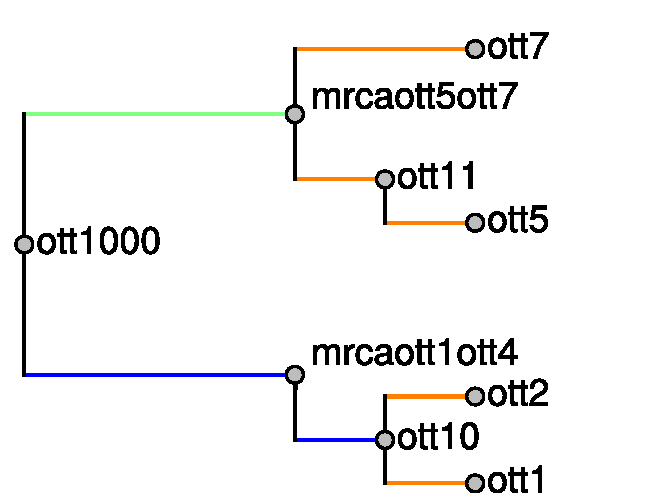
\includegraphics[scale=0.5]{annotation_example__induced1_color}%
\end{minipage}

}

\bigskip{}

\bigskip{}

\hfill{}\subfloat[JSON annotations relating edges of (c) to edges of (a)]{%
\shadowbox{\begin{minipage}[t]{1.0\columnwidth}%
\texttt{\{}

\texttt{~~\textquotedbl{}nodes\textquotedbl{}: \{}

\texttt{~~~~\textquotedbl{}mrcaott1ott4\textquotedbl{}: \{ \textquotedbl{}}\texttt{\textcolor{blue}{partial\_path\_of}}\texttt{\textquotedbl{}: \{
\textquotedbl{}tree1\textquotedbl{}: \textquotedbl{}node15\textquotedbl{},
... \} \},}

\texttt{~~~~\textquotedbl{}ott10\textquotedbl{}:~~~~~~~~~\{
\textquotedbl{}}\texttt{\textcolor{blue}{partial\_path\_of}}\texttt{\textquotedbl{}: \{
\textquotedbl{}tree1\textquotedbl{}: \textquotedbl{}node15\textquotedbl{},
... \} \},}

\texttt{~~~~\textquotedbl{}mrcaott5ott7\textquotedbl{}: \{ \textquotedbl{}\textcolor{mylime}{supported\_by}\textquotedbl{}:~~~
\{ \textquotedbl{}tree1\textquotedbl{}: \textquotedbl{}node16\textquotedbl{},
... \} \},}

\texttt{~~~~\textquotedbl{}ott1\textquotedbl{}:~~~~~~~~~~\{
\textquotedbl{}}\texttt{\textcolor{orange}{terminal}}\texttt{\textquotedbl{}: ~~~~~~~\{
\textquotedbl{}tree1\textquotedbl{}: \textquotedbl{}ott1\textquotedbl{},
... ~~\} \},}

\texttt{~~~~\textquotedbl{}ott2\textquotedbl{}:~~~~~~~~~~\{
\textquotedbl{}}\texttt{\textcolor{orange}{terminal}}\texttt{\textquotedbl{}: ~~~~~~~\{
\textquotedbl{}tree1\textquotedbl{}: \textquotedbl{}ott2\textquotedbl{},
... ~~\} \},}

\texttt{~~~~\textquotedbl{}ott5\textquotedbl{}:~~~~~~~~~~\{
\textquotedbl{}}\texttt{\textcolor{orange}{terminal}}\texttt{\textquotedbl{}: ~~~~~~~\{
\textquotedbl{}tree1\textquotedbl{}: \textquotedbl{}ott5\textquotedbl{},
... ~~\} \},}

\texttt{~~~~\textquotedbl{}ott11\textquotedbl{}:~~~~~~~~~\{
\textquotedbl{}}\texttt{\textcolor{orange}{terminal}}\texttt{\textquotedbl{}: ~~~~~~~\{
\textquotedbl{}tree1\textquotedbl{}: \textquotedbl{}ott5\textquotedbl{},
... ~~\} \},}

\texttt{~~~~\textquotedbl{}ott7\textquotedbl{}:~~~~~~~~~~\{
\textquotedbl{}}\texttt{\textcolor{orange}{terminal}}\texttt{\textquotedbl{}: ~~~~~~~\{
\textquotedbl{}tree1\textquotedbl{}: \textquotedbl{}ott7\textquotedbl{},
... ~~\} \}}

\texttt{~~\},}

\texttt{~~...}

\texttt{\} }%
\end{minipage}}

}\hfill{}

\caption{\label{fig:displayed-annotations}The relationship of edges in summary
tree $\protect\summaryTree$ (b) to edges in the input tree $T_{1}$
(a). Only edges of $\protect\summaryTree$ that are present in the
induced tree $\protect\summaryTree(1)$ are represented by JSON annotations
(d). Taxon names are here suppressed in favor of OTT IDs, and edges
are referenced via their tipward nodes. Edges in $\protect\summaryTree(1)$
that correspond to terminal edges of $T_{1}$ are orange; edges of
$\protect\summaryTree(1)$ that are supported by edges of $T_{1}$
are blue; where multiple edges of $\protect\summaryTree(1)$ correspond
to the same edge of $T_{1}$ they are green. There is no conflict
in this example. Also, if this were output from propinquity, then
each internal node of $\protect\summaryTree$ would be supported by
other inputs trees that are not shown here. }
\end{figure}


To reveal the connections between the groupings found in the a summary
supertree and the input trees, propinquity uses a few Python scripts
and the \texttt{otc-annotate-synth} tool from otcetera to create an
annotations file describing the pipeline used and the connections
between phylogenetic information in the inputs and the summary.  The
JSON file produced by \texttt{otc-annotate-synth} encodes a ``nodes''
property that holds a mapping between a node name for the summary
tree (using the naming convention described in the previous section)
and a node provenance object that categorizes the relationship between
the node and the inputs. The node provenance object for node $x$
uses several properties to categorize the relationship between the
node and the inputs; each property in the node provenance object maps
to a structure storing the tree ID and node IDs for the input tree
nodes. 

Conceptually, this annotation operation is equivalent to considering
every node $j$ in each input tree $i$ and the summary tree node
$x$. Because the vast majority of nodes in the input studies will
be compatible but not directly relevant to node $x$ we do not list
all of the compatible groupings. If node $x$ is not included in the
induced tree $\mathcal{\mathbb{S}}(i)$, then none of the nodes of
tree $i$ will be referred to in the annotations for node $x$. Even
if $x$ is included in $\mathcal{\mathbb{S}}(i)$, many of the nodes
of $T_{i}$ will be compatible with $x$ while being relevant to other
parts of the summary tree. The only input nodes listed for node $x$
are with rooted taxon bipartitions which conflict with, are displayed
by, or are resolved by the the rooted taxonomic bipartition associated
with node $x$. All input nodes that cannot be displayed by any supertree
that contains $x$ are stored in a ``\conflictswith{}'' property
of the node provenance object. If node $j$ of $T_{i}$ is displayed
by the summary tree and $x$ is part of the path of $\mathcal{\mathbb{S}}(i)$
that displays the split between descendants of $j$ and other taxa,
then a reference to the node $j$ will be in the node provenance object.
The exact categorization of this annotation will depend on the configuration
of node $x$ on the induced tree $\mathcal{\mathbb{S}}(i)$:
\begin{itemize}
\item if $x$ is on a terminal path in the induced tree then node $j$ will
be listed in the ``\terminal{}'' property;
\item if $x$ is along an internal path that contains some nodes with out-degree
equal to 1, then node $j$ will be listed in the ``\partialpathof{}''
property; and
\item if $x$ is along an internal path without any node of out-degree 1,
then node $j$ will be listed in the ``\supportedby{}'' property,
because node $j$ supports the existence of grouping $x$ in the sense
that collapsing the edge that separates $x$ from its parent would
cause the summary tree to no longer display node $j$.
\end{itemize}
These three relationships are illustrated in Figure \ref{fig:displayed-annotations}.
Finally, if $T_{i}$ does not display $x$ from $\mathcal{\mathbb{S}}(i)$,
but there exists an unresolved node $j$ in $T_{i}$ which could be
resolved such that the tree would then display $x$, then a reference
to node $j$ will be listed in the ``\resolves{}'' property of node
$x$. 

The otcetera annotation tool can also detect cases in which including
information from node $j$ in $T_{i}$ could further resolve a polytomy
$x$ in the summary tree; such a case would be annotated using the
``\resolvedby{}'' property of $x$. However, because of our goal
of excluding unnecessary polytomies, none of the nodes in propinquity's
summary tree will use this annotation when they are annotated with
the set of input trees.

\subsubsection{Self-documentation}

An optional step in the propinquity pipeline (triggered by the executing
the ``make html'' target) can compose an ``index.html'' file for
each directory created during the pipeline to explain the artifacts
held in that directory and report summary statistics about the summarization
run.

\section{Results}

We seek to assess the performance of our new supertree method by
comparing it to the supertree method of \cite{HinchliffEtAl2015}.  The
method of \cite{HinchliffEtAl2015} was used to construct the Open Tree
of Life v4 (\otl{}).  Therefore, in order to facilitate comparison, we 
applied our method to the same input trees and taxonomy used by
\otl{}.  
We refer to the resulting supertree as \otlprop{} since it was
constructed by applying the propinquity pipeline to the same inputs as
\otl{}.

\subsection{Inputs}

The flag-cleaned version of OTT used in the construction of both
supertrees contained 2,424,255 leaves.  The
\otl{} supertree was constructed from 482 phylogenetic inputs,
containing a total of 45,385 leaves, of which 41,029 were unique.
After flag-cleaning and exemplification by propinquity, these trees contained 40,323
unique tips. We used the same cleaning flags to trim the taxonomy and
input trees when constructing \otlprop{}, so \otl{} and \otlprop{} contain the
same number of leaves.

\subsection{Subproblems}
In the \otlprop{} summary tree, the decomposition procedure produced
5,406 subproblems, but only 1,422 of these were non-trivial to solve.
If a subproblem contains only two tips it is trivial; 2,362 subproblems
were trivial in this way. Similarly, if a subproblem contains only
2 trees it is trivial to solve because the solution will simply be
all of the groupings from the first tree combined with all of the
groupings from the second tree that are compatible with the first
tree; 3,052 subproblems were trivial in this way. The subproblem with
the largest number of tips contained 946 tips. The largest subproblem,
in terms of the number of input trees (including the taxonomic tree)
that were relevant, had 16 trees. Without decomposition, the supertree
problem would have had 482 input trees and 41,226 leaves.


% table

% outputs - representation of input trees
% outputs - annotations

% conflicts in v4: 2,760
% conflicts in v4propr: 1,357

% displayed in v4: 35,518
% displayed in v4prop: 39,639


% # of input splits represented by v4, but not v4prop
% # of input splits represented by v4prop, but not v4
% # of input splits represented by v4 and v4prop

\begin{table}

\caption{Representation of input splits in the \otl{} tree and the \otlprop{} tree.}
\resizebox{\textwidth}{!}{%
\begin{tabular}{lcccccc}
 & \supportedby{} & \partialpathof{} & \terminal{} & \conflictswith{} & \resolvedby{} & \resolves{}\tabularnewline
\hline 
\otl{} & 34,595 & 923 & 45,385 & 2,760 & 2,718 & 473\tabularnewline
\hline 
\otl{} only & 745 & 54 & 0 & 2,055 & 2,718 & 0\tabularnewline
\hline 
\otlprop{} & 38,521 & 1,118 & 45,385 & 1,357 & 0 & 515\tabularnewline
\hline 
\otlprop{} only & 4,671 & 249 & 0 & 652 & 0 & 42\tabularnewline
\hline
\label{tab:representinputs}
\end{tabular}}


\end{table}

\begin{table}

\caption{Representation of taxonomy splits in the \otl{} tree and the \otlprop{} tree.}
\resizebox{\textwidth}{!}{%
\begin{tabular}{lcccccc}
 & \supportedby{} & \partialpathof{} & \terminal{} & \conflictswith{} & \resolvedby{} & \resolves{}\tabularnewline
\hline 
\otl{} & 125,384 & 0 & 2,424,255 & 1,998 & 4 & 3,676\tabularnewline
\hline 
\otl{} only & 296 & 0 & 0 & 19 & 4 & 17\tabularnewline
\hline 
\otlprop{} & 125,107 & 0 & 2,424,255 & 2,279 & 0 & 3,883\tabularnewline
\hline 
\otlprop{} only & 19 & 0 & 0 & 300 & 0 & 224\tabularnewline
\hline 
\label{tab:representtaxonomy}
\end{tabular}}


\end{table}

\subsection{Representing input splits}

We performed an annotation of both the \otl{} tree and the \otlprop{}
tree as described in section \ref{sec:Annotation} to assess the
ability of our new supertree method to represent splits from input
phylogenies.  Table \ref{tab:representinputs} classifies the input
phylogeny splits according to how they relate to a summmary tree, so
that each input edge falls in one of \supportedby{}, \partialpathof{},
\terminal{}, \conflictswith{}, or \resolvedby{}. For example, the
numbers in the \conflictswith{} column indicate the number of input
splits $j$ with at least one summary edge $x$ such that the relation
``$x$ \conflictswith{} $j$'' holds.  The total number of non-terminal
input phylogeny splits considered was 40,996.

The number of displayed input splits (\supportedby{}
+ \partialpathof{}) increased from 35,518 (for \otl{}) to 39,639 (for \otlprop{});
an 11\% increase. When examining which splits are displayed, we find
that the \otlprop{} tree displays 4,920 input splits that
are not displayed by the \otl{} tree, whereas the \otl{} tree displays
only 799 input splits that are not displayed by the \otlprop{} tree.  The number of input
splits that conflict with the summary (\conflictswith{}) dropped from
2,760 to 1,357, a decrease of 1,403, or 51\%.  In accordance with the
goal of not containing unnecessary polytomies, the number of input
splits that do not conflict with the summary tree, but are not
incorporated (\resolvedby{}) dropped from 2,718 to 0.  We also find that
the number of polytomies in input phylogenies that are resolved by the
summary tree increases from 473 for \otl{} to 515 for \otlprop{}.

We also performed an annotation of the \otl{} tree and the \otlprop{}
tree to assess the degree to which these trees represent taxonomy
splits (Table \ref{tab:representtaxonomy}).  The \otlprop{} tree
conflicts with 281 more taxonomy splits than the \otl{} tree.  Since
the taxonomy is the lowest ranked input tree, this increased conflict
with the taxonomy is an expected result of incorporating more splits
from higher-ranked input phylogenies.  


\section{Conclusions}

Here we have described the motivation and methodology used by our new
supertree method that is currently used by the Open Tree of Life
project to build summary supertrees on the scale of millions of leaves.
Our new method represented 11\% more input phylogeny splits with 51\%
less conflict compared to the Open Tree of Life version 4 summary
tree, when applied to the same inputs. Unlike the previous method
\citep{HinchliffEtAl2015}, our new method is guaranteed to incorporate
input splits unless they conflict with the summary tree. The method is
implemented in the Open Source software package propinquity.  A
modified version of the treemachine software which built the summary
tree described in the \citet{HinchliffEtAl2015} paper is used by the
project to serve the tree produced by propinquity via Open Tree of
Life APIs.

The migration of summary tree construction from treemachine (used for
version 4) to propinquity (for all versions from v5.0 to present) has
increased the pace of synthesis tree releases from the Open Tree of
Life project.  This is partly because the newly available annotations
feature has made it possible to identify which input trees are
responsible for taxa being included or excluded from the summary tree.
Additionally, the new propinquity software pipeline has decreased the decreased
the computational time required to construct a supertree from several
hours to about 8 minutes (after some preprocessing steps which only
have to be performed when the input taxonomy changes).  The amount of
RAM required during tree construction has also decreased substantially. 

\section{Acknowledgements}

Thanks to Emily Jane McTavish, Karen Cranston, Jonathan Rees, Jim Allman, Cody Hinchliff,
Stephen Smith, and Joseph Brown for discussions and feedback. Thanks
to NSF grant 1208393 (DEB), part of the collaborative Open Tree of
Life awards, the University of Kansas, and the Heidelberg Institute
for Theoretical Studies for funding.

\bibliographystyle{upmplainnat}
\bibliography{otcetera}


\appendix

\section{The maximum sum displayed groups' weighted scores criterion}\label{sec:The-maximum-sum}

Let $\mathcal{W}$ is a weighting function that maps any input tree's
internal node to a non-negative number. If $I(\mathbb{S},i,j)$ is
an indicator function that is 1 if summary tree $\mathbb{S}$ displays
the node $V(i,j)$ and 0 otherwise then: $SDGWS(\mathbb{S})=\sum_{i}\sum_{j}I(\mathbb{S},i,j)\mathcal{W}(i,j)$
is the ``sum of displayed groups' weighted scores'' for a tree where
$i$ indexes all of the input trees and $j$ indexes each non-root
internal node in tree $i$. Preference for this tree is referred to
as the maximum sum displayed groups' weighted scores criterion (MSDGWS
criterion). The summary tree constructed by the propinquity pipeline
is a greedy heuristic for finding a tree that maximizes this score
when the weights for a node are determined by the tree's weight and
the difference in weighting is so large that displaying one node from
a highly ranked tree is preferred to displaying all of the nodes in
the trees with lower rank.

\section{Description of the decomposition algorithm of otc-uncontested-decompose}\label{sec:Decompose-algorithm}

The input is the a ranked list of input trees and comprehensive taxonomy. 

\subsection{Creation of multigraph of the taxonomy with embedded trees}

The tool creates a multigraph by starting with a graph isomorphic
to the taxonomic tree. The nodes and edges created in this step will
be referred to as the ``taxonomic graph.'' Next, we add nodes and
edges to that graph in a procedure that we refer to as ``embedding''
the input trees into the taxonomy. A node is introduced for each node
in an input tree, and these nodes are mapped the MRCA nodes in the
taxonomic graph. In other words, for any node $y$ in an input tree
with a cluster of descendants, $\mathcal{C},$ we find the most tipward
node $z$ in the taxonomic graph that is an ancestor to all of the
taxa in $\mathcal{C}$; let $m(y)=z$ refer to this mapping, and $m^{\prime}(z)=y$
refer to the reverse mapping. Each edge $e_{ij}$ in a source tree
$i$ connects ancestor to its descendant, $a(e_{ij})\rightarrow d(e_{ij})$.
The edges are introduced into the graph. We also introduce new edges
to create a from $m(a(e_{ij}))$ through its descendants to $m(d(e_{ij}))$;
we denote this path $p(e_{ij})$ and refer to the edges in the path
as ``embedding edges for tree $i$''. Note, that this is a path
through the taxonomic nodes, while the edge $e_{ij}$ connects source
tree nodes. The mapping between $e_{ij}$ and $p(e_{ij})$ is stored,
and the edges are labelled with the index $i$ so that it is clear
which tree created them. Because the taxonomic tree is highly unresolved,
it is frequently the case that $m(a(e_{ij}))$ is the same node as
$m(d(e_{ij}))$; in these cases the embedding edge is a loop. This
situation occurs whenever edge $e_{ij}$ can resolve part of the polytomy
represented by a taxon. 

We treat the taxonomy as the lowest ranked input tree. The next step
will collapse contested edges in the taxonomic graph. To retain all
of the information from the taxonomy we embed the taxonomy into the
taxonomic graph as if it were another input tree

\subsection{Detection of uncontested higher taxa}

After every input tree and the taxonomy tree have been embedded into
the taxonomic graph, we perform postorder traversal over the taxonomic
graph that underlies the multi-graph. For any internal node (each
of which corresponds to a non-terminal taxon) we determine whether
or not it is contested by examining each input tree. We can determine
tree $i$ contests the taxon represented by taxonomic node $x$ by
looking at the parents of all of the ``exiting'' embedding edges
for tree $i$. These are the set of embedding edges that have $x$
as a daughter and have a parent node that is not $x$ (ergo a parent
node that is taxonomically higher than $x$). If there are more than
one parent nodes in this set of exiting embedding edges, then tree
$i$ contests that taxon. If there is only one parent node, then the all
of the constituent taxa belonging to this taxon that are present in
tree $i$ have one parent that is more inclusive; this means that
the input tree does not contest monophyly of the taxon.

If the taxon is uncontested, then it may be the case that some input
trees do not contest the taxon, but contain polytomies that could
be resolved to display the taxon. The cases can be identified by finding
multiple exiting embedding edges that have the same taxon $y$ as
their parent node. In these cases, a pseudo input tree node is created
and becomes the parent node for these edges; this new node is then
connected to $y$ as if it had been an input edge. This operation
is equivalent to resolving an input tree's polytomy in favor of the
monophyly of the uncontested taxon. This is the only way in which
the input trees are modified during the decomposition.

\subsection{Collapsing contested taxa from the taxonomic graph}

If a taxonomic node $x$ fails the ``uncontested'' test described
in the previous section, then the node corresponding to the taxon
is removed from the taxonomic graph and the set of edges (and mappings
between input edges and embedded paths) is updated as if this taxon
had not been present in when the taxonomic graph was created. This
consists of detecting changing any edge in an embedding path that
is adjacent to $x$ by replacing the reference to $x$ with a reference
to its parent $a(x)$. Note that we do not collapse the edge corresponding
to this taxon in the part of the graph that represents the embedding
of the taxonomy into the taxonomic graph. Thus, the taxonomy will
still claim the monophyly of the taxon. This is relevant if the input
grouping that contests taxon $x$ is overruled (in the subproblem
solution step) by a higher ranked split. In other words, the fact
that the a taxon is contested during the decomposition is not a guarantee
that the taxon will not be monophyletic in the final supertree.

\subsection{Emitting subproblems}

Whenever an uncontested taxon is identified, the appropriate slice
of each input trees that intersect with the taxon is written to a
file. Then the multigraph is simplified by slicing any off the taxon.
This slicing is accomplished by examing all of the exiting embedding
edges for the taxon. The descendant taxa of each input tree is relabeled
with the identifier of the contested taxa and all of that node's descendants
are removed. Thus this input node will act as as if it were a leaf
mapped to the uncontested taxon. All descendants of the taxonomic
graph are also pruned off.
\end{document}
